\chapter{Javadoc}
\label{javadoc}

\index{comment!end-of-line}
\index{comment!multi-line}
\index{comment!documentation}

Java programs have three different types of comments:

\begin{enumerate}
\item {\bf End-of-line comments} (\java{//}), which generally contain short phrases that explain specific lines of code.

\item {\bf Multi-line comments} (with \java{/*} at the beginning and \java{*/} at the end), which are typically only used for copyright statements at the top of the file.

\item {\bf Documentation comments} (with \java{/**} at the beginning and \java{*/} at the end), which describe what each class and method does.
\end{enumerate}

End-of-line and multi-line comments are written primarily for yourself.
They help you remember specific details about your source code.
Documentation comments, on the other hand, are written for others.
They explain how to use your classes and methods in other programs.

\index{HTML}
\index{Javadoc}

A nice feature of the Java language is the ability to embed documentation in the source code itself.
That way, you can write it as you go, and as things change, it is easier to keep the documentation consistent with the code.

You can extract documentation from your source code, and generate well-formatted HTML pages, using a tool called {\bf Javadoc}.
This tool is included with the Java compiler, and it is widely used.
In fact, the official documentation for the Java library (see~\url{https://thinkjava.org/apidoc}) is generated by Javadoc.


\section{Reading Documentation}

\index{documentation}

%One of the nice things about Java is that it comes with an extensive library of classes and methods.
%But before you use them, you might have to read the documentation.
%And sometimes that's not easy.

As an example, let's look at the documentation for \java{Scanner}, a class we first used in Section~\ref{scanner}.
You can find the documentation quickly by doing a web search for ``Java Scanner''.
Figure~\ref{fig.scanner} shows a screenshot of the page.

\begin{figure}[!ht]
\begin{center}
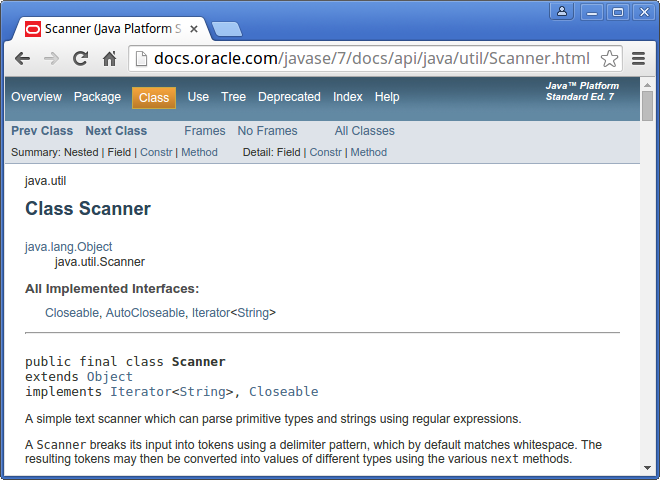
\includegraphics[width=0.9\textwidth]{figs/scanner.png}
\caption{Screenshot of the documentation for \java{Scanner}.}
\label{fig.scanner}
\end{center}
\end{figure}

Documentation for other classes uses a similar format.
The first line is the package that contains the class, such as \java{java.util}.
The second line is the name of the class.
The ``Implemented Interfaces'' section lists some of the functionality a \java{Scanner} has.
%; we won't say more about that for now.

%The next two lines indicate that every \java{Scanner} is also an \java{Object}; that will make more sense after Section~\ref{inheritance}.

The next section of the documentation is a narrative that explains the purpose of the class and includes examples of how to use it.
This text can be difficult to read, because it may use terms you have not yet learned.
But the examples are often very useful.
A good way to get started with a new class is to paste the examples into a test file and see if you can compile and run them.

One of the examples shows how you can use a \java{Scanner} to read input from a \java{String} instead of \java{System.in}:

%NOTE: only use of Scanner w/o System.in; mention this again in String chapter?
\begin{code}
String input = "1 fish 2 fish red fish blue fish";
Scanner s = new Scanner(input);
\end{code}

After the narrative, code examples, and some other details, you will find the following tables:

\begin{description}

\item[Constructor summary:]
Ways of creating, or ``constructing'', a \java{Scanner}.

\item[Method summary:]
The list of methods that the \java{Scanner} class provides.

\item[Constructor detail:]
More information about how to create a \java{Scanner}.

\item[Method detail:]
More information about each method.

\end{description}

For example, here is the summary information for \java{nextInt}:

\begin{stdout}
public int nextInt()
Scans the next token of the input as an int.
\end{stdout}

\index{signature}

The first line is the method's {\bf signature}, which specifies the name of the method, its parameters (none), and what type it returns (\java{int}).
The next line is a short description of what it does.

The ``Method detail'' explains more:

\begin{stdout}
public int nextInt()
Scans the next token of the input as an int.

An invocation of this method of the form nextInt() behaves in
exactly the same way as the invocation nextInt(radix), where
radix is the default radix of this scanner.

Returns:
the int scanned from the input

Throws:
InputMismatchException - if the next token does not match
    the Integer regular expression, or is out of range
NoSuchElementException - if input is exhausted
IllegalStateException - if this scanner is closed
\end{stdout}

The ``Returns'' section describes the result when the method succeeds.
In contrast, the ``Throws'' section describes possible errors and exceptions that may occur.
Exceptions are said to be ``thrown'', like a referee throwing a flag, or like a toddler throwing a fit.

It might take you some time to get comfortable reading documentation and learning which parts to ignore.
But it's worth the effort.
Knowing what's available in the library helps you avoid reinventing the wheel.
And a little bit of documentation can save you a lot of debugging.


\section{Writing Documentation}

As you benefit from reading good documentation, you should ``pay it forward'' by writing good documentation.

\index{comment!documentation}
\index{documentation!Javadoc comments}

Javadoc scans your source files looking for documentation comments, also known as ``Javadoc comments''.
They begin with \java{/**} (two stars) and end with \textcolor{comment}{\tt */} (one star).
Anything in between is considered part of the documentation.

Here's a class definition with two Javadoc comments, one for the \java{Goodbye} class and one for the \java{main} method:

\begin{code}
/**
 * Example program that demonstrates print vs println.
 */
public class Goodbye {

    /**
     * Prints a greeting.
     */
    public static void main(String[] args) {
        System.out.print("Goodbye, ");  // note the space
        System.out.println("cruel world");
    }
}
\end{code}

The class comment explains the purpose of the class.
The method comment explains what the method does.

Notice that this example also has an end-of-line comment (\java{//}).
In general, these comments are short phrases that help explain complex parts of a program.
They are intended for other programmers reading and maintaining the source code.

In contrast, Javadoc comments are longer, usually complete sentences.
They explain what each method does, but they omit details about how the method works.
And they are intended for people who will use the methods without looking at the source code.

Appropriate comments and documentation are essential for making source code readable.
And remember that the person most likely to read your code in the future, and appreciate good documentation, is you.


\section{Javadoc Tags}

%In Section~\ref{sec:javadoc}, we discussed how to write documentation comments using \java{/**}.
It's generally a good idea to document each class and method, so that other programmers can understand what they do without having to read the code.

\index{tag}
\index{param tag}
\index{return tag}
\index{documentation!Javadoc tags}

To organize the documentation into sections, Javadoc supports optional {\bf tags} that begin with the at sign (\java{@}).
For example, we can use \java{@author} and \java{@version} to provide information about the class.

\begin{code}
/**
 * Utility class for extracting digits from integers.
 *
 * @author Chris Mayfield
 * @version 1.0
 */
public class DigitUtil {
\end{code}

\index{description}

Documentation comments should begin with a {\bf description} of the class or method, followed by the tags.
These two sections are separated by a blank line (not counting the \textcolor{comment}{\tt *}).

For methods, we can use \java{@param} and \java{@return} to provide information about parameters and return values.

\begin{code}
/**
 * Tests whether x is a single digit integer.
 *
 * @param x the integer to test
 * @return true if x has one digit, false otherwise
 */
public static boolean isSingleDigit(int x) {
\end{code}

\index{HTML}
\index{Javadoc}

Figure~\ref{fig.javadoc} shows part of the resulting HTML page generated by Javadoc.
Notice the relationship between the Javadoc comment (in the source code) and the resulting documentation (in the HTML page).

\begin{figure}[!ht]
\begin{center}
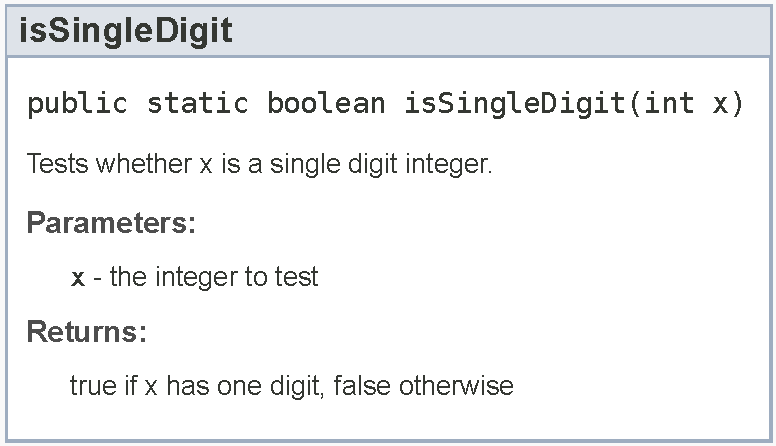
\includegraphics[width=298pt]{figs/javadoc.pdf}
\caption{HTML documentation for \java{isSingleDigit}.}
\label{fig.javadoc}
\end{center}
\end{figure}

When writing parameter comments, do not include a hyphen (\java{-}) after the \java{@param} tag.
Otherwise, you will have two hyphens in the resulting HTML documentation.

Notice also that the \java{@return} tag should not specify the type of the method.
Comments like \textcolor{comment}{\tt @return boolean} are not useful, because you already know the return type from the method's signature.

Methods with multiple parameters should have separate \java{@param} tags that describe each one.
Void methods should have no \java{@return} tag, since they do not return a value.
Each tag should be on its own line in the source code.


\section{Example Source File}

Now let's take a look at a more complete example.
The code for this section is in the {\tt appb} directory of {\tt ThinkJavaCode2}.
See page~\pageref{code} for instructions on how to download the repository.

Professional-grade source files often begin with a copyright statement.
This text spans multiple lines, but it is not part of the documentation.
So we use a multi-line comment (\java{/*}) rather than a documentation comment (\java{/**}).
Our example source file, {\tt Convert.java}, includes the MIT License (\url{https://opensource.org/licenses/MIT}).

\index{Convert.java}

\begin{scriptsize}
\begin{code}
/*
 * Copyright (c) 2019 Allen Downey and Chris Mayfield
 *
 * Permission is hereby granted, free of charge, to any person obtaining a copy
 * of this software and associated documentation files (the "Software"), to deal
 * in the Software without restriction, including without limitation the rights
 * to use, copy, modify, merge, publish, distribute, sublicense, and/or sell
 * copies of the Software, and to permit persons to whom the Software is
 * furnished to do so, subject to the following conditions:
 *
 * The above copyright notice and this permission notice shall be included in
 * all copies or substantial portions of the Software.
 *
 * THE SOFTWARE IS PROVIDED "AS IS", WITHOUT WARRANTY OF ANY KIND, EXPRESS OR
 * IMPLIED, INCLUDING BUT NOT LIMITED TO THE WARRANTIES OF MERCHANTABILITY,
 * FITNESS FOR A PARTICULAR PURPOSE AND NONINFRINGEMENT. IN NO EVENT SHALL THE
 * AUTHORS OR COPYRIGHT HOLDERS BE LIABLE FOR ANY CLAIM, DAMAGES OR OTHER
 * LIABILITY, WHETHER IN AN ACTION OF CONTRACT, TORT OR OTHERWISE, ARISING FROM,
 * OUT OF OR IN CONNECTION WITH THE SOFTWARE OR THE USE OR OTHER DEALINGS IN THE
 * SOFTWARE.
 */
\end{code}
\end{scriptsize}

%This program uses a \java{Scanner}, so we have to \java{import} it.
Import statements generally follow the copyright text.
After that, we can define the class itself and begin writing the documentation (\java{/**}).

\begin{code}
import java.util.Scanner;

/**
 * Methods for converting to/from the metric system.
 *
 * @author Allen Downey
 * @author Chris Mayfield
 * @version 6.1.5
 */
public class Convert {
\end{code}

A common mistake that beginners make is to put \java{import} statements between the documentation and the \java{public class} line.
Doing so separates the documentation from the class itself.
To avoid this issue, always make the end of the comment (the \textcolor{comment}{\tt */}) ``touch'' the word \java{public}.


This class has two constants and three methods.
The constants are self-explanatory, so there is no need to write documentation for them.

\begin{code}
public static final double CM_PER_INCH = 2.54;

public static final int IN_PER_FOOT = 12;
\end{code}

The methods, on the other hand, could use some explanation.
Each documentation comment includes a description, followed by a blank line, followed by a \java{@param} tag for each parameter, followed by a \java{@return} tag.

\begin{code}
/**
 * Converts a measurement in centimeters to inches.
 *
 * @param cm length in centimeters
 * @return length in inches
 */
public static double toImperial(double cm) {
    return cm / CM_PER_INCH;
}

/**
 * Converts a length in feet and inches to centimeters.
 *
 * @param feet how many feet
 * @param inches how many inches
 * @return length in centimeters
 */
public static double toMetric(int feet, int inches) {
    int total = feet * IN_PER_FOOT + inches;
    return total * CM_PER_INCH;
}
\end{code}

The \java{main} method has a similar documentation comment, except there is no \java{@return} tag since the method is \java{void}.
%And because it's longer than a few lines, it includes end-of-line comments (\java{//}) as well.

\begin{code}
/**
 * Tests the conversion methods.
 *
 * @param args command-line arguments
 */
public static void main(String[] args) {
    double cm, result;
    int feet, inches;
    Scanner in = new Scanner(System.in);

    // test the Imperial conversion
    System.out.print("Exactly how many cm? ");
    cm = in.nextDouble();
    result = toImperial(cm);
    System.out.printf("That's %.2f inches\n", result);
    System.out.println();

    // test the Metric conversion
    System.out.print("Now how many feet? ");
    feet = in.nextInt();
    System.out.print("And how many inches? ");
    inches = in.nextInt();
    result = toMetric(feet, inches);
    System.out.printf("That's %.2f cm\n", result);
}
\end{code}

Here are two ways you can run the Javadoc tool on this example program:

\begin{enumerate}

\index{command-line interface}

\item From the command line, go to the location for {\tt Convert.java}.
The {\tt -d} option of {\tt javadoc} indicates where to generate the HTML files.

\begin{stdout}
javadoc -d doc Convert.java
\end{stdout}

\item From DrJava, click the {\sf Javadoc} button on the toolbar.
The IDE will then prompt you for a location to generate the HTML files.
\end{enumerate}

For more examples of what you can do with Javadoc comments, see the source code of any Java library class (e.g., {\tt Scanner.java}).
Section~\ref{src.zip} explains how to find the source files for the Java library on your computer.


\section{Vocabulary}

\begin{description}

\term{documentation}
Comments that describe the technical operation of a class or method.

\term{Javadoc}
A tool that reads Java source code and generates documentation in HTML format.

\term{signature}
The first line of a method that defines its name, return type, and parameters.

\term{tag}
A label that begins with an at sign (\java{@}) and is used by Javadoc to organize documentation into sections.

\term{description}
The first line of a documentation comment that explains what the class/method does.

\end{description}
